\documentclass[12pt,a4paper,notitlepage]{scrreprt}
\usepackage{amssymb}
\usepackage{amsmath}
\usepackage{verbatim, fontenc}
\usepackage{tabulary, float}
\usepackage[locale = DE,space-before-unit=true,per-mode = symbol]{siunitx}
\usepackage{icomma}
\usepackage{booktabs,multirow}
\usepackage[breaklinks=true,colorlinks=true,linkcolor=blue,urlcolor=blue,citecolor=blue]{hyperref}
\usepackage[autostyle]{csquotes}
\usepackage{wrapfig}
\usepackage[format=plain]{caption}
\usepackage{eurosym}
\usepackage[ngerman]{babel}
\usepackage[backend=biber,style=numeric,sorting=none]{biblatex}
\usepackage{gensymb}
\DeclareMathOperator{\sinc}{sinc}
\DeclareSIUnit{\dBm}{dBm}
\DeclareSIUnit[per-mode=reciprocal]\WN{\per\centi\meter}
\usepackage{chngcntr}
\usepackage{graphicx,subcaption}
\usepackage[normalem]{ulem}
\useunder{\uline}{\ul}{}
\usepackage[table,xcdraw]{xcolor}




\titlehead{\includegraphics[width=5cm]{logo.jpg}}

\title{\centering Solarpotential Agrivoltaics Bericht}
\author{Luis Reitmeier\thanks{\href{mailto:reitmeierluis@icloud.com}{reitmeierluis@icloud.com}}}
\date{\today}

\begin{document}

\counterwithout{footnote}{chapter}

\maketitle

\vfill
    \section*{Abstract}
    Während der Stromverbrauch in Tirol weiterhin steigt, wird die Produktion von erneuerbaren energien aufgrund ausgeschöpfter Potentiale in der Wasserkraft und mangelnden Freiflächen für Solar verlangsamt. Agrivoltaics hat es sich zum Ziel gemacht, die vielen Landwirtschaftlichen Flächen zusäzlich als Solarflächen zu nutzen. Das ist nicht nur wegen der ganzjährigen Stromproduktion von Vorteil, sondern hilft auch gegen Wetterereignisse wie Hagel, Starkregen, Trockenheit und Hitze oder zu starke Sonneneinstrahlung. Dieser Bericht gibt eine komplette Kosten/ Nutzenübersicht über das Potenzial ihrer Fläche, und legt die gesammte Leistung die wir ihnen bringen können näher.



\thispagestyle{empty}

\tableofcontents

\thispagestyle{empty}
\cleardoublepage
\pagenumbering{arabic}
\newpage

\chapter{Potentialanalyse}

Im folgenden wird das Potential analysiert. Bei einer Fläche von 14ha

\begin{figure}
    \centering
    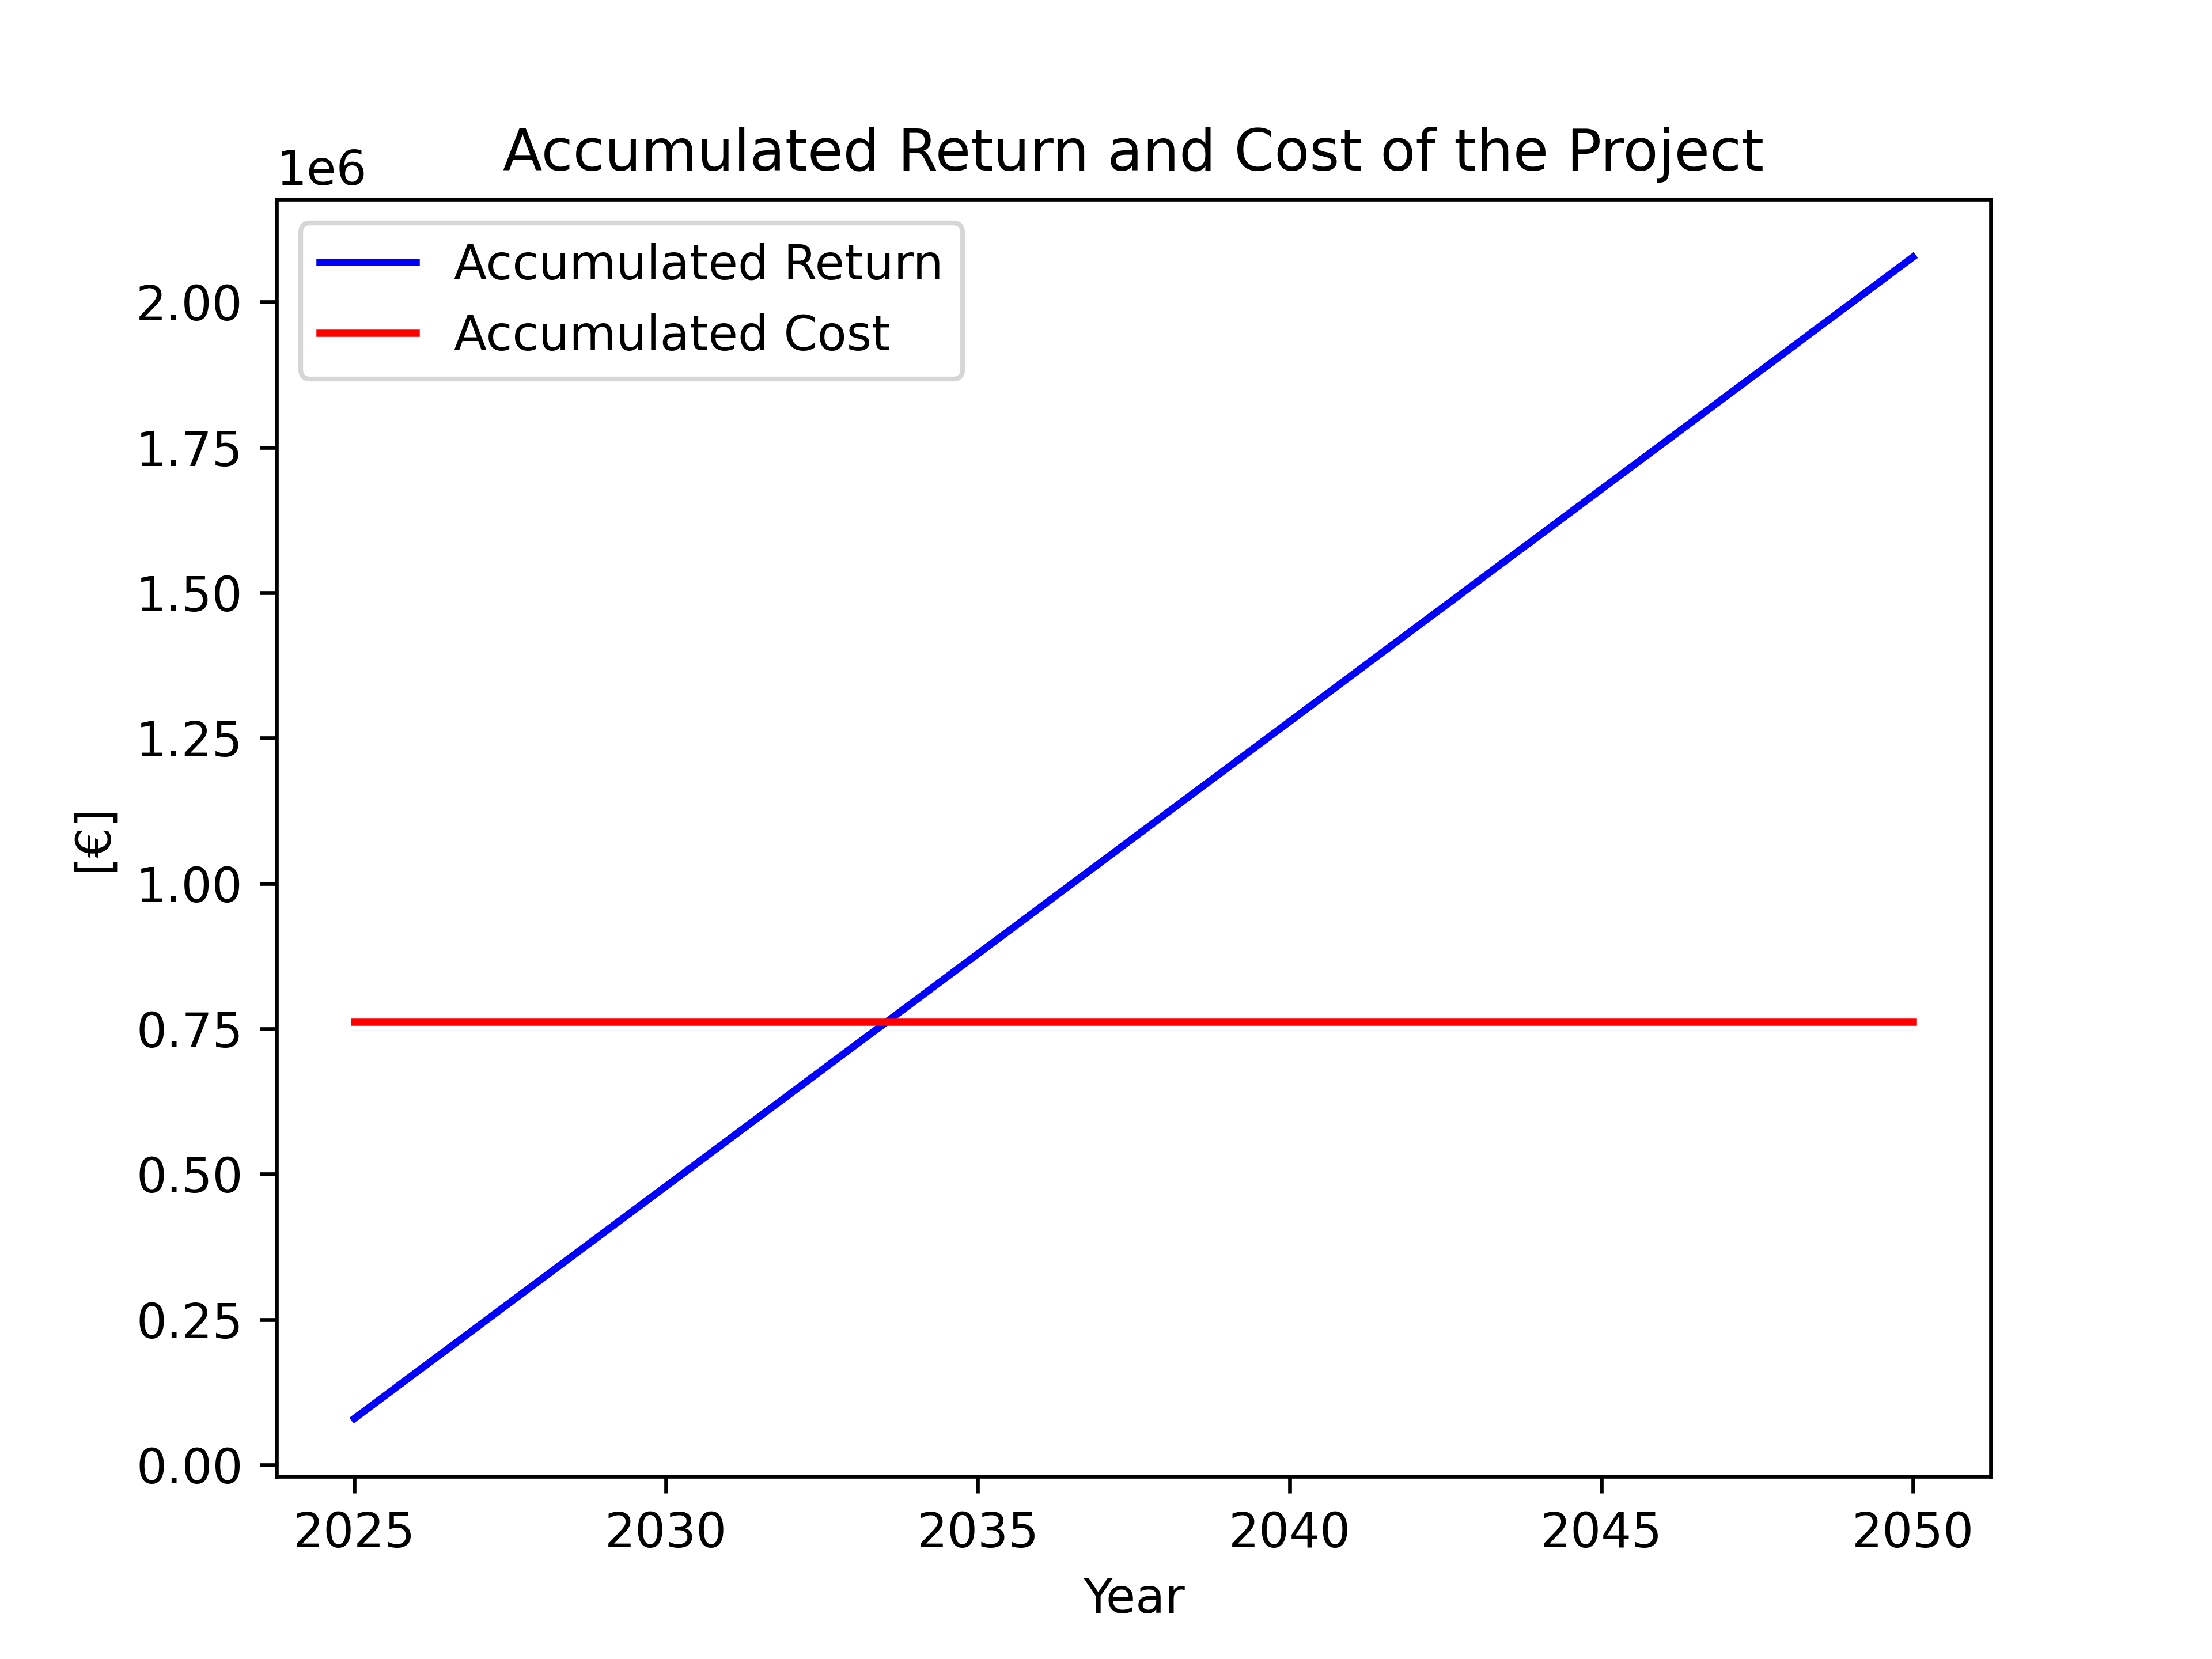
\includegraphics[scale=0.7]{images/Akkumulierter_Ertrag.png}
    \caption{Der Ertrag in Euro von 2025 bis 2050. Die Projektkosten sind mit der Roten linie eingetragen}
    \label{Projektkosten}
\end{figure}

Und nun zu den Monaten

\begin{figure}
    \centering
    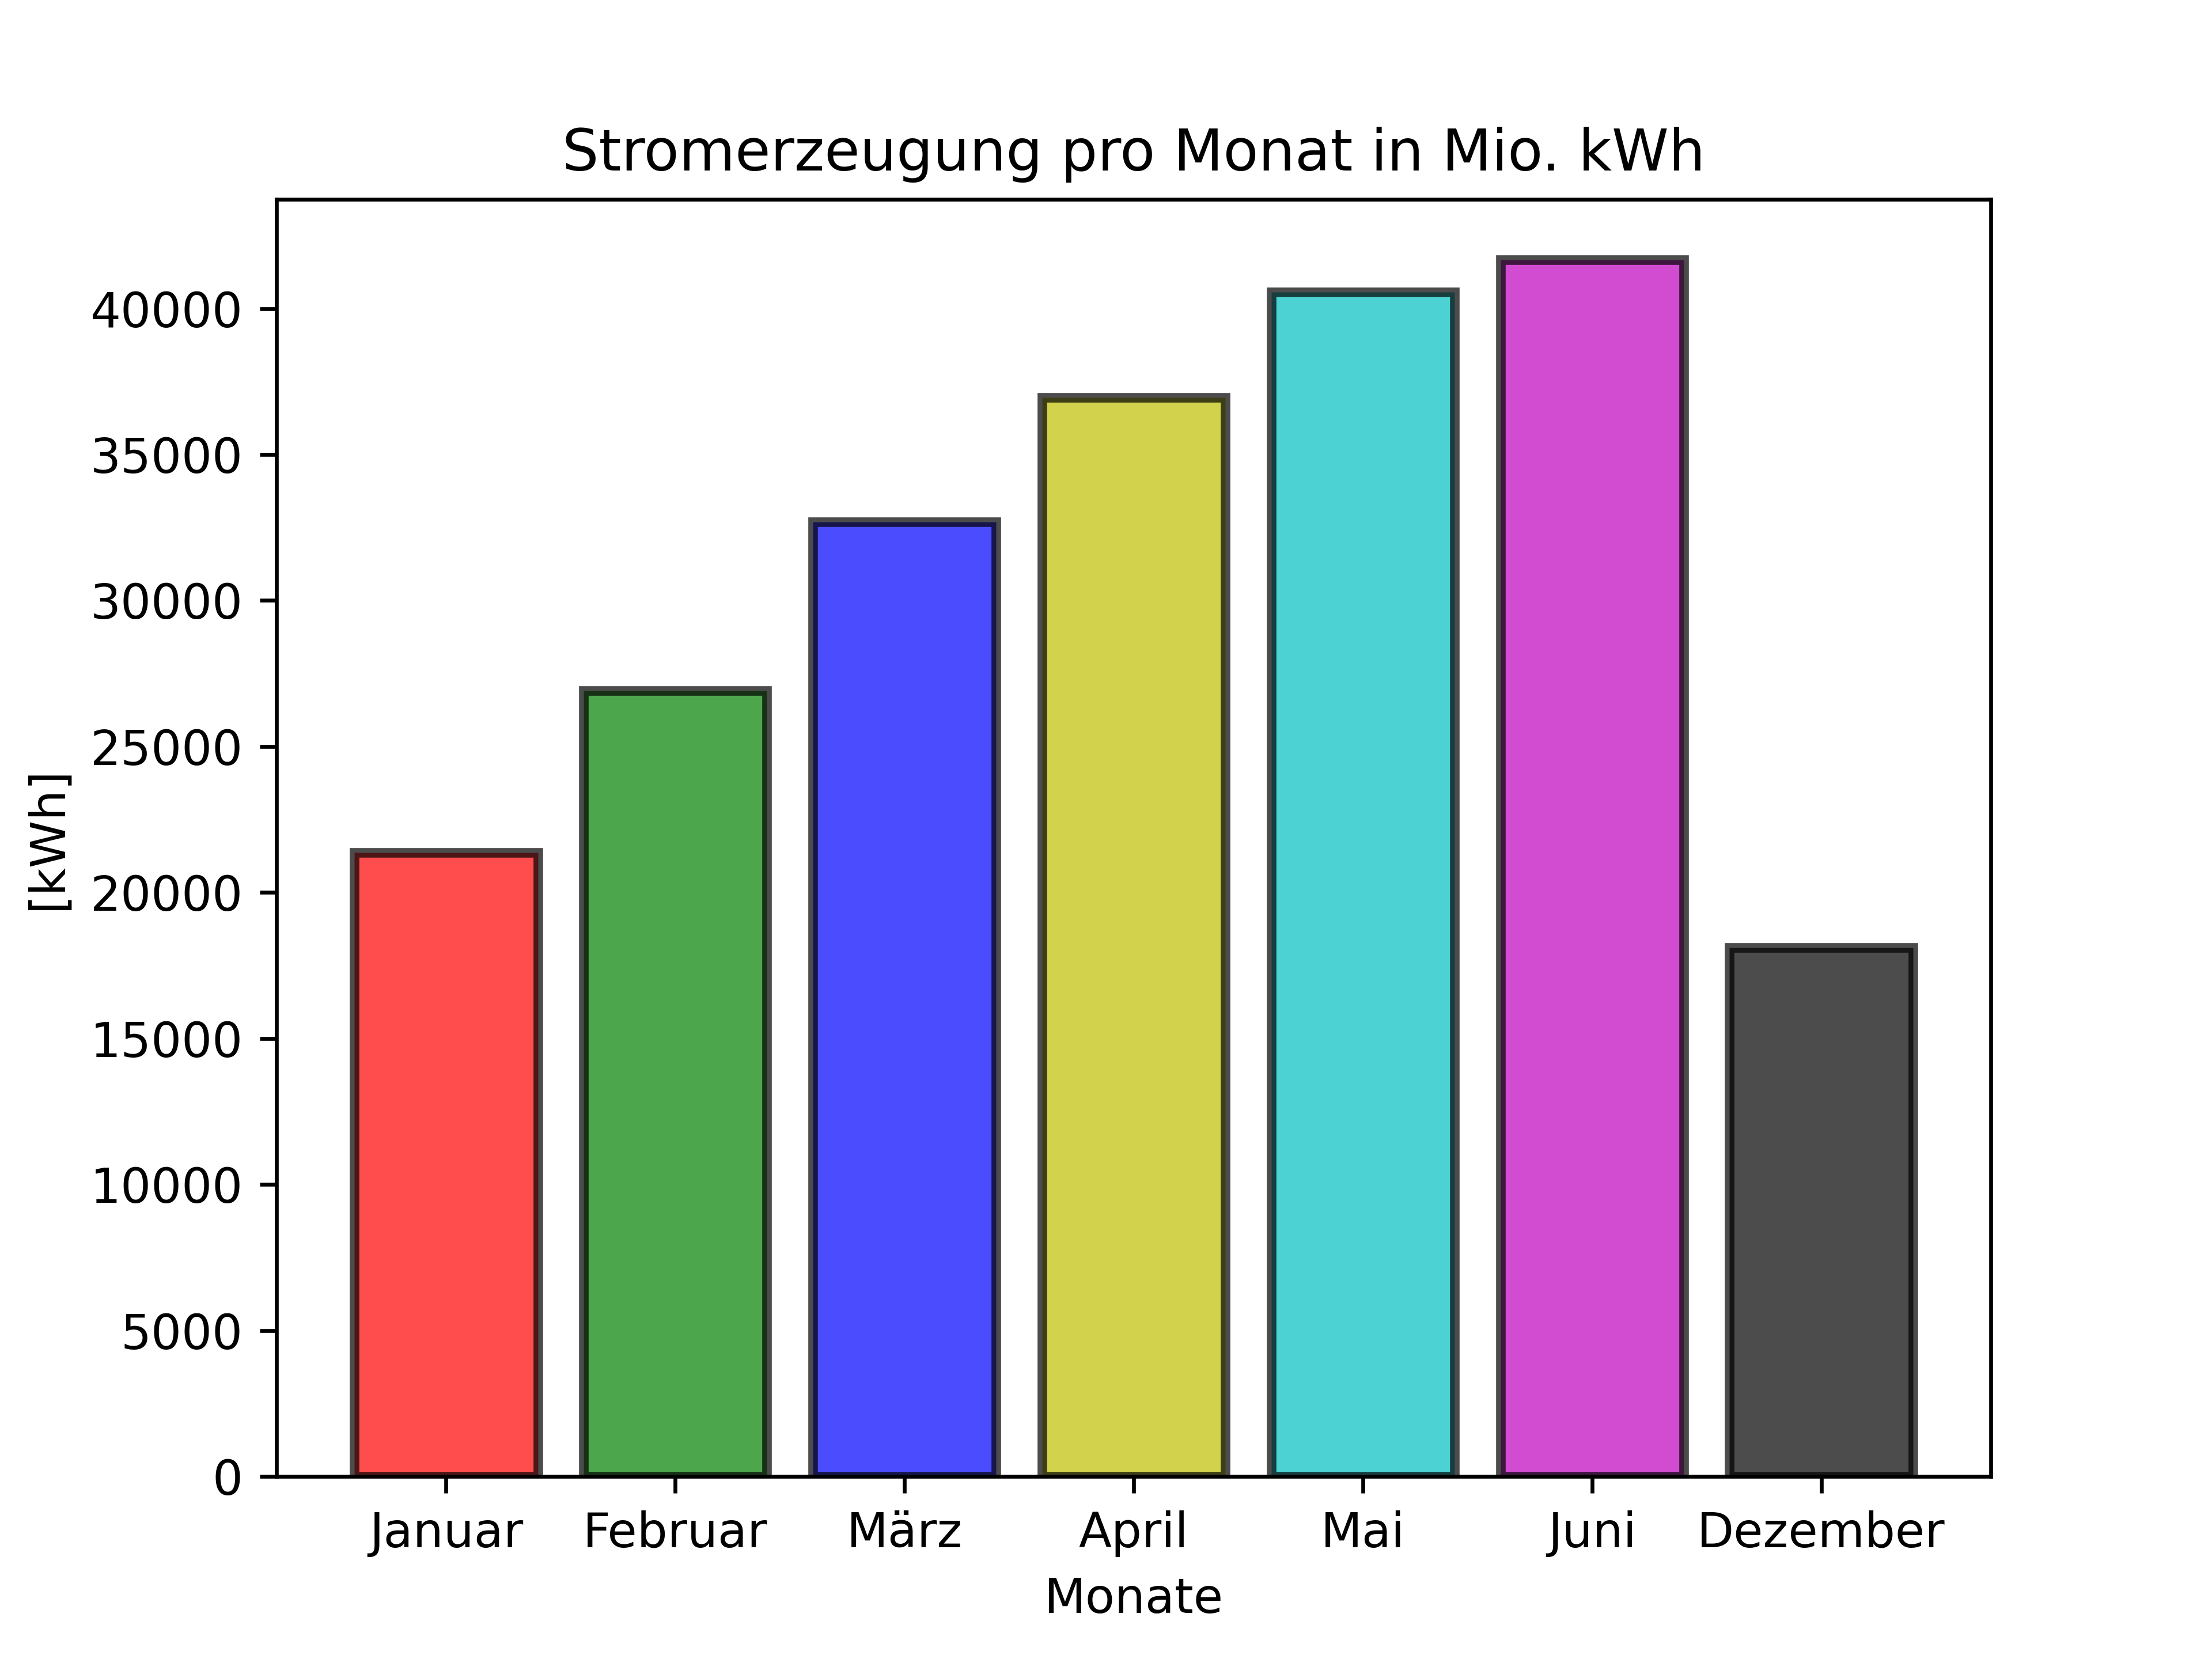
\includegraphics[scale=0.7]{images/Stromerzeugung_pro_Monat.png}
    \caption{Stromerzeugung pro Monat für die Monate, in welchen Daten vorhanden sind}
    \label{Stromerzeugung}
\end{figure}



\end{document}

